% !Mode:: "TeX:UTF-8"
\def\usewhat{pdflatex}                               % 定义编译方式 dvipdfmx 或者 pdflatex,默认为 dvipdfmx
                                                     % 方式编译,如果需要修改,只需改变花括号中的内容即可。
%\documentclass[12pt,openany,oneside]{book}

\documentclass[a4paper, 11pt]{article}                                                   % 本科生毕业论文通常采用单页排版
\usepackage{pdfpages}
\usepackage{float}
\usepackage{wrapfig}

%\usepackage{indentfirst}

%\usepackage{graphicx}
%\usepackage{caption}
%\usepackage{subcaption}
%\usepackage{subfigure}

%\makeatletter
%\let\c@subfigure\relax
%\let\l@subfigure\relax
%\makeatother

%\usepackage{epstopdf}


% !Mode:: "TeX:UTF-8"
%  Authors: 张井   Jing Zhang: prayever@gmail.com     天津大学2010 级管理与经济学部信息管理与信息系统专业硕士生
%           余蓝涛 Lantao Yu: lantaoyu1991@gmail.com  天津大学2008 级精密仪器与光电子工程学院测控技术与仪器专业本科生

%%%%%%%%%% Package %%%%%%%%%%%%
\usepackage{graphicx}                       % 支持插图处理
\usepackage[a4paper,text={146.4true mm,239.2 true mm},top= 26.2true mm,left=31.8 true mm,head=6true mm,headsep=6.5true mm,foot=16.5true mm]{geometry}
                                            % 支持版面尺寸设置
\usepackage[squaren]{SIunits}               % 支持国际标准单位

\usepackage{titlesec}                       % 控制标题的宏包
\usepackage{titletoc}                       % 控制目录的宏包
\usepackage{fancyhdr}                       % fancyhdr宏包 支持页眉和页脚的相关定义
\usepackage[UTF8]{ctex}                     % 支持中文显示
\usepackage{CJKpunct}                       % 精细调整中文的标点符号
\usepackage{color}                          % 支持彩色
\usepackage{amsmath}                        % AMSLaTeX宏包 用来排出更加漂亮的公式
\usepackage{amssymb}                        % 数学符号生成命令
\usepackage[below]{placeins}    %允许上一个section的浮动图形出现在下一个section的开始部分,还提供\FloatBarrier命令,使所有未处理的浮动图形立即被处理
\usepackage{multirow}                       % 使用Multirow宏包,使得表格可以合并多个row格
\usepackage{booktabs}                       % 表格,横的粗线;\specialrule{1pt}{0pt}{0pt}
\usepackage{longtable}                      % 支持跨页的表格。
\usepackage{tabularx}                       % 自动设置表格的列宽

%\makeatletter
%\let\c@subfigure\relax
%\makeatother

\usepackage{subfigure}                      % 支持子图 %centerlast 设置最后一行是否居中
\usepackage[subfigure]{ccaption}            % 支持子图的中文标题
\usepackage[sort&compress,numbers]{natbib}  % 支持引用缩写的宏包
\usepackage{enumitem}                       % 使用enumitem宏包,改变列表项的格式
\usepackage{calc}                           % 长度可以用+ - * / 进行计算
\usepackage{txfonts}                        % 字体宏包
\usepackage{bm}                             % 处理数学公式中的黑斜体的宏包
\usepackage[amsmath,thmmarks,hyperref]{ntheorem}  % 定理类环境宏包,其中 amsmath 选项用来兼容 AMS LaTeX 的宏包
\usepackage{CJKnumb}                        % 提供将阿拉伯数字转换成中文数字的命令
\usepackage{indentfirst}                    % 首行缩进宏包
\usepackage{CJKutf8}                        % 用在UTF8编码环境下,它可以自动调用CJK,同时针对UTF8编码作了设置
%\usepackage{hypbmsec}                      % 用来控制书签中标题显示内容
\newcommand{\tabincell}[2]{\begin{tabular}{@{}#1@{}}#2\end{tabular}}
\usepackage{xcolor}
%支持代码环境
\usepackage{listings}
\lstset{numbers=left,
language=[ANSI]{C},
numberstyle=\tiny,
extendedchars=false,
showstringspaces=false,
breakatwhitespace=false,
breaklines=true,
captionpos=b,
keywordstyle=\color{blue!70},
commentstyle=\color{red!50!green!50!blue!50},
frame=shadowbox,
rulesepcolor=\color{red!20!green!20!blue!20}
}
%支持算法环境
\usepackage[boxed,ruled,lined]{algorithm2e}
\usepackage{algorithmic}

\usepackage{array}
\newcommand{\PreserveBackslash}[1]{\let\temp=\\#1\let\\=\temp}
\newcolumntype{C}[1]{>{\PreserveBackslash\centering}p{#1}}
\newcolumntype{R}[1]{>{\PreserveBackslash\raggedleft}p{#1}}
\newcolumntype{L}[1]{>{\PreserveBackslash\raggedright}p{#1}}

% 生成有书签的 pdf 及其生成方式。通常可以在 tjumain.tex 文件的第一行选择 pdflatex 或者是 dvipdfmx 编译手段。如果选择前者,则使用 pdflatex + pdflatex 编译; 如果选择后者,在编译的时候选择 latex + bibtex + latex + latex 编译。出现混淆的时候,系统会报错。
% 如果您的pdf制作中文书签有乱码使用如下命令,就可以解决了
\def\atemp{dvipdfmx}\ifx\atemp\usewhat
\usepackage[dvipdfmx,unicode,               % dvipdfmx 编译, 加入了中文复制,粘贴支持引擎。
            pdfstartview=FitH,
            bookmarksnumbered=true,
            bookmarksopen=true,
            colorlinks=false,
            pdfborder={0 0 1},
            citecolor=blue,
            linkcolor=red,
            anchorcolor=green,
            urlcolor=blue,
            breaklinks=true
            ]{hyperref}
\fi

\def\atemp{pdflatex}\ifx\atemp\usewhat
\usepackage{cmap}                           % pdflatex 编译时,可以生成可复制、粘贴的中文 PDF 文档, 缺点是在Windows上显示时效果不大好,字体发虚
\usepackage[pdftex,unicode,
            %CJKbookmarks=true,
            bookmarksnumbered=true,
            bookmarksopen=true,
            colorlinks=false,
            pdfborder={0 0 1},
            citecolor=blue,
            linkcolor=red,
            anchorcolor=green,
            urlcolor=blue,
            breaklinks=true
            ]{hyperref}
\fi
                                % 定义本文所使用宏包
\graphicspath{{figures/}}                            % 定义所有的 .eps 文件在 figures 子目录下
\begin{document}                                     % 开始全文

\begin{CJK*}{UTF8}{song}
\begin{center}

  \begin{figure}[h]
  \centering
  
\includegraphics[width=0.7\textwidth]{figures/ustc}
  \end{figure}

\vspace*{25pt}
{ \fontsize{20pt}{24pt}\selectfont{\textbf{“大学生创新训练计划”项目结题报告}}}

\vspace*{20pt}

\begin{center}
  \begin{tabular}{lclc}
    中文题目 &  \underline{基于SDN的云中大数据网络优化的研究} \\
    英\qquad 文& \underline{ Research of bigdata network optimization} \\
    题\qquad 目& \underline{based on SDN in cloud computing} \\
    学\qquad 院& \underline{信息学院} \\
    指导教师 &  \underline{张文逸} \\
    \end{tabular}
    \vspace*{50pt}
    \begin{tabular}{lclc}
    小组成员: \\
    姓\qquad 名& \underline{孟思尧} & 学\qquad 号 & \underline{PB12210076} \\
    姓\qquad 名& \underline{王笑霄} & 学\qquad 号 & \underline{PB12210100} \\
    姓\qquad 名& \underline{张广帅}  & 学\qquad 号 & \underline{PB12210080} \\
  \end{tabular}
\end{center}

  \vspace*{25pt}
  \today

\end{center}
\clearpage
\begin{center}
  { \fontsize{15pt}{18pt}\selectfont{\textbf{摘\qquad 要}}}
\end{center}

{ \fontsize{10pt}{15pt}\selectfont{\textbf{关键词:}}}云计算,大数据,SDN,HADOOP,网络优化
\clearpage
\begin{center}
  { \fontsize{15pt}{18pt}\selectfont{\textbf{ABSTRACT}}}
\end{center}

{ \fontsize{10pt}{15pt}\selectfont{\textbf{KEY WORDS:}}}Cloud computing,Bigdata,SDN,HADOOP,network optimization
\clearpage
\tableofcontents
%\part{问题阐述}
%\chapter{问题阐述}
\section{项目背景}
\subsection{项目的意义和关键问题}
大数据应用正深刻改变人们的生活,已经成为当前学术界、工业界的关注焦点。大数据应用开发云平台纷纷推出大数据计算框架。如Amazon的EC2,微软的Azure。虽然云平台上的大数据框架方便了第三方开发者和用户,但其性能上还存在较多问题,尤其是网络的问题。在2014 Daytona GraySort排序赛上,基于Spark的系统它使用了207个EC2 节点在23分钟内排序了100TB的数据而夺冠。而上届冠军Hadoop用了2100台Yahoo内置的机器,花了72分钟,这性能提升不言而喻!更重要的是这次比赛证实Shuffle真正的瓶颈在于网络。传统大数据网络架构是数据库服务器将应用服务器请求的数据通过网络传输到应用服务器上,处理后,将改写的数据再写回数据库服务器,而且处理过程中会出现大量的中间结果也需要网络传输。当数据量较大时,很可能堵塞网络。因而对于进一步提升大数据处理性能,研究云平台上大数据网络问题显得尤为重要。\\
\subsection{研究方向}
\begin{description}
  \item[软件定义网络(SDN)] 软件定义网络(SDN)是当前和未来网络研究的一个重要方向,通过将网络的数据转发层和逻辑控制层分离,提高了网络的灵活性和可编程性。可以在控制层面设计应用感知的控制策略,如网络接入、数据转发路由、流量工程等,从而提高应用的性能。因此,我们拟通过SDN来优化云平台上大数据框架的网络性能。
  \item[coflow调度] 考虑到当前数据中心用并行计算的框架处理大规模的数据,充分考虑数据流的相关性(coflow),设计调度算法
\end{description}
\section{项目平台的选择}
\subsection{Hadoop}
\subsubsection{为什么选择Hadoop}
数据并行计算框架很多,如:Mapreduce,Spark,Google Dataflow等等,我们为什么选择Hadoop?
首先,认识一下Hadoop,Hadoop是一种计算集群,它将数据分析的工作分配到多个集群节点上,从而并行处理数据。经过调研,Hadoop用于大数据处理,主要有如下几个优势:
\begin{description}
  \item[1、灵活的可扩展性] 要充分利用大数据最大的优势就需要实时或接近实时地对海量数据进行分析处理。大数据分析面临的一个巨大的难题是数据量的不断增加。而Hadoop集群的并行处理能力能明显提高分析速度,但随着要分析的数据量的增加,集群的处理能力会受到影响。Hadoop通过增加集群节点,可以线性地扩展集群以处理更大的数据集。另外,在集群负载下降时,也可以减少节点,以高效使用计算资源。所以Hadoop的弹性很好
  \item[2、Hadoop的设计适合大数据处理] 大数据一般都是分布广泛的并且是非结构化的。而Hadoop非常适合处理这类数据,因为Hadoop的mapreduce的计算框架工作原理是将数据拆分成片,并将每个“分片”分配到特定的集群节点上进行分析。数据不必均匀分布,因为每个数据分片都是在独立的集群节点上进行单独处理。
  \item[3、Hadoop成本低] Hadoop的软件是开源的,同时,Hadoop支持商用硬件,可以运行在一般商业机器构成的大型集群上,如:亚马逊弹性计算云(Amazon EC2)等,不必花费重金购买服务器级别的硬件设备。所以我们可以低成本的实现计算能力强大的Hadoop集群,性价比很高。
  \item[4、容错能力强] 在Hadoop集群进行大数据处理分析过程中,当一个数据分片发送到某个节点进行分析时,该数据在集群其它节点上会存有副本。通过备份的方式,即使一个节点发生故障,数据可以快速的恢复,继续进行分析处理。故障检测和自动恢复是Hadoop最初的设计目标,所以Hadoop很健壮。
\end{description}
由于Hadoop具有上述优势,使得Hadoop在学术界和工业界都大受欢迎。\\
\subsubsection{Mapreduce计算框架}
Mapreduce是什么?怎样完成大数据处理?\\
Hadoop的设计思路源于Google的GFS和MapReduce。它是一个开源软件框架,通过在集群计算机中使用MapReduce这个简单的编程模型,可编写和运行分布式应用程序处理大规模数据。

\begin{figure}[!htb]
    \centering
    \let\c@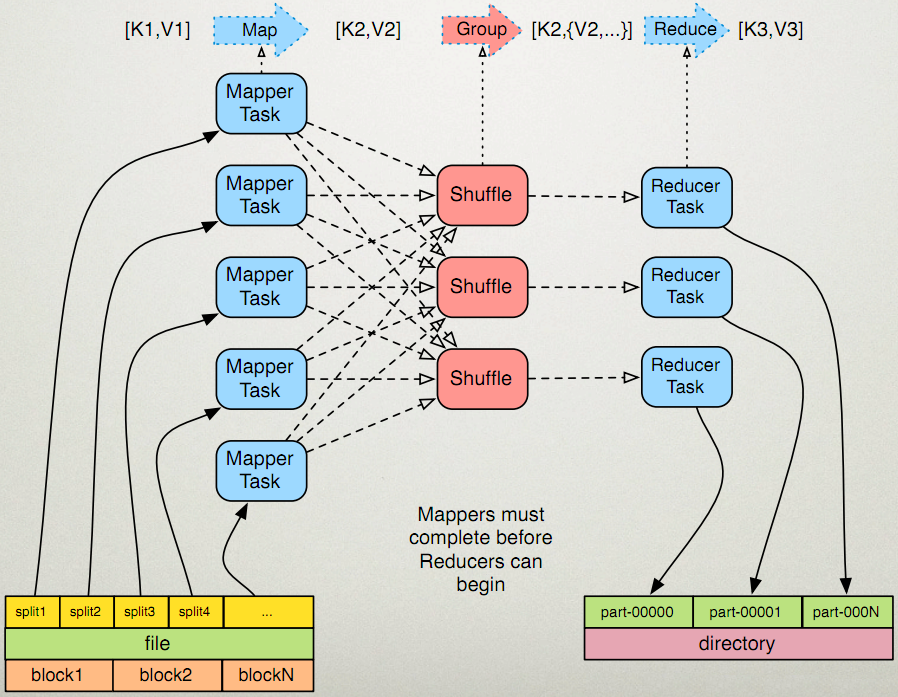
\includegraphics[height=2in]{mapreduce.png}\relax
    \caption{Mapreduce计算框架}
\end{figure}
MapReduce架构的大数据处理的操作流程如下:
\begin{enumerate}
  \item 首先调用MapReduce库的输入流模块,将输入文件分成M个数据片度,每个数据片段的大小可以通过可选的参数来控制。然后用户程序在机群中创建大量的程序副本。程序副本中包含一个特殊的master程序。其它的程序都是worker程序,由master分配任务。有M个Map任务和R个Reduce任务将被分配,master将一个Map任务或Reduce任务分配给一个空闲的worker。
  \item 被分配了map任务的worker程序读取相关的输入数据片段,从输入的数据片段中解析出key/value pair,然后把key/value pair传递给用户自定义的Map函数,由Map函数生成并输出的中间key/value pair,并缓存在内存中。
  \item 缓存中的key/value pair通过调用Partition模块分成R个区域,之后周期性的写入到本地磁盘上。缓存的key/value pair 在本地磁盘上的存储位置将被传给master,由master负责把这些存储位置再传送给Reduce worker。
  \item 当Reduce worker程序接收到master程序发来的数据存储位置信息后,使用RPC从Map worker所在主机的磁盘上读取这些缓存数据。当Reduce worker读取了所有的中间数据后,通过对key进行排序后使得具有相同key值的数据聚合在一起。由于许多不同的key值会映射到相同的Reduce 任务上,因此必须进行排序。如果中间数据太大无法在内存中完成排序,那么就要在外部进行排序。
  \item Reduce worker程序遍历排序后的中间数据,对于每一个唯一的中间key值,Reduce worker程序将这个key值和它相关的中间value值的集合传递给用户自定义的Reduce函数。Reduce函数的输出被追加到所属分区的输出文件。
  \item 当所有的Map和Reduce任务都完成之后,master唤醒用户程序。在这个时候,在用户程序里的对MapReduce调用才返回。在成功完成任务之后,MapReduce的输出存放在R个输出文件中(对应每个Reduce任务产生一个输出文件,文件名由用户指定)。一般情况下,用户不需要将这R个输出文件合并成一个文件–他们经常把这些文件作为另外一个MapReduce的输入,或者在另外一个可以处理多个分割文件的分布式应用中使用。
\end{enumerate}

\subsubsection{Shuffle阶段}
整体的Shuffle过程包含以下几个部分:Map端Shuffle、Sort阶段、Reduce 端Shuffle。即是说:Shuffle 过程横跨 map 和 reduce 两端,中间包含 sort 阶段。

\begin{figure}[!htb]
    \centering
    \let\c@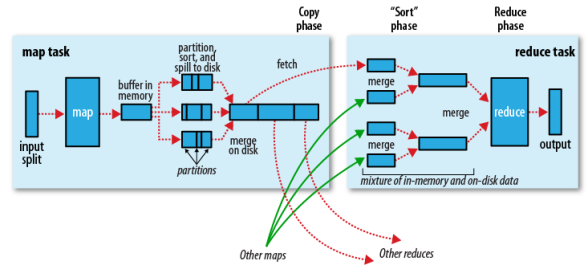
\includegraphics[height=2in]{shuffle.png}\relax
    \caption{shuffle阶段}
\end{figure}
 在Hadoop集群中,大部分map task与reduce task的执行是在不同的节点上,Reducer通过HTTP方式得到map阶段输出文件的分区,所以很多情况下Reduce 执行时需要跨节点去拉取其它节点上的map task结果。在Mapreduce的Shuffle阶段,如果集群正在运行的 job 有很多,而且需要跨节点拉取数据时,会产生大量的数据在网络中传输,对集群内部的网络资源消耗会很严重,尽可能地减少对带宽的不必要消耗,并且保证完整地从map task 端拉取数据到reduce端。
\subsection{SDN}
\subsubsection{Floodlight}
SDN(软件定义网络)利用OpenFlow协议,把路由器的控制平面(control plane)从数据平面(data plane)中分离出来,以软件方式实现。这个架构可以让网络管理员,在不改动硬件设备的前提下,通过集中式的控制器(Controller)以标准化的接口对各种网络设备进行管理和配置,那么这将为网络资源的设计、管理和使用提供更多的可能性,为控制网络流量提供了新的方法。\\
控制器作为SDN网络中的重要组成部分,我们选择Floodlight作为SDN控制器。因为Floodlight是目前主流的SDN控制器之一,它的稳定性、易用性已经得到SDN专业人士一致好评,由于其完全开源,这让SDN网络世界变得更加有活力。能集中地灵活控制SDN网络,为核心网络及应用创新提供了良好的扩展平台。\\
Floodlight控制器是一个企业级的,使用Java开发的OpenFlow协议的控制器。OpenFlow是一个由Open Networking Foundation (ONF)管理的开放标准。它定义了一种协议让远程控制器通过路由器可以修改网络设备的行为,使用定义良好的转发指令集。Floodlight被设计为同支持OpenFlow标准的设备(交换机,路由器,虚拟交换机)一起工作。\\
Floodlight controller模块为多数应用实现了一些通用的功能:

\begin{enumerate}
  \item 发现网络状态和事件(拓扑结构,设备,流量)
  \item 能够控制网络交换机(network switches)通信
  \item 管理floodlight模块,共享存储,线程,测试等资源
  \item 提供一个web界面和debug服务器(Python)
\end{enumerate}
\begin{figure}[!htb]
    \centering
    \let\c@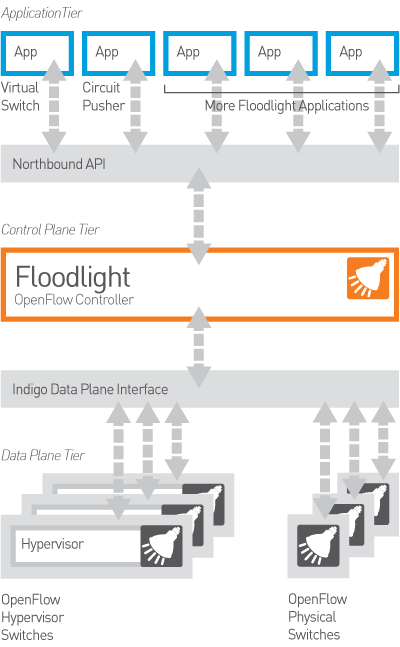
\includegraphics[height=2.5in]{project_floodlight_infographic.png}\relax
    \caption{Floodlight控制器架构图}
\end{figure}
Floodlight控制器工作过程如下:
\begin{enumerate}
  \item 控制器与交换机建立ofchannel通道,控制器通过ofchannel 控制和管理交换机。
  \item 当交换机收到一个数据包且流表中没有匹配条目,交换机会将数据包封装在packet-in消息发送给控制器,此时数据包会缓存在交换机中等待处理。
  \item 控制器收到packet-in消息后,可以发送flow-mod消息向交换机写一个流表项,并且将flow-mod消息中buffer-id字段设置为packet-in消息中的buffer-id值。从而控制器向交换机写入了一条与数据包相关的流表项,并且指定该数据包按照该流表项的action列表处理。但是并不是所有的数据包都需要向交换机中添加一条流表项来匹配处理,网络中还存在多种数据包,它出现的数量很少(如ARP,IGMP 等),以至于没有必要通过流表项来指定这一类数据包的处理法,此时控制器可以使用packet-out消息,告诉交换机某一个数据包如何处理。
\end{enumerate}
\subsubsection{OVS}
Open vSwitch是一个由Nicira Networks主导的开源项目,通过运行在虚拟化平台上的虚拟交换机,为本台物理机上的VM提供二层网络接入, 跟云中的其它物理交换机一样工作在Layer 2层。Open vSwitch充分考虑了在不同虚拟化平台间的移植性,采用平台无关的C语言开发。并且遵循Apache2.0许可;我们有传统的物理交换机,为什么还要开发Open vSwitch呢?\\
在传统数据中心中,网络管理员习惯了每台物理机的网络接入均可见并且可配置。通过在交换机某端口的策略配置,可以很好控制指定物理机的网络接入,访问策略,网络隔离,流量监控,数据包分析,Qos 配置,流量优化等。但是在云平台上,如果没有网络虚拟化技术的支持,管理员只能看到被桥接的物理网卡,其上川流不息地跑着n台VM 的数据包。仅凭物理交换机支持,管理员无法区分这些包属于哪个OS 哪个用户。而且难以满足以下需求:
\begin{description}
  \item[网络隔离] 物理网络管理员早已习惯了把不同的用户组放在不同的VLAN中,例如研发部门、销售部门、财务部门,做到二层网络隔离。Open vSwitch通过在host上虚拟出一个软件交换机,等于在物理交换机上级联了一台新的交换机,所有VM通过级联交换机接入,让管理员能够像配置物理交换机一样把同一台host上的众多VM分配到不同VLAN中去;
  \item[QoS配置] 在共享同一个物理网卡的众多VM中,我们期望给每台VM配置不同的速度和带宽,以保证核心业务VM的网络性能。通过在Open vSwitch端口上,给各个VM配置QoS,可以实现物理交换机的traffic queuing和traffic shaping功能。
  \item[流量监控] 物理交换机通过xxFlow技术对数据包采样,记录关键域,发往Analyzer处理。进而实现包括网络监控、应用软件监控、用户监控、网络规划、安全分析、会计和结算、以及网络流量数据库分析和挖掘在内的各项操作。例如,NetFlow流量统计可以采集的数据非常丰富,包括:数据流时戳、源IP地址和目的IP地址、 源端口号和目的端口号、输入接口号和输出接口号、下一跳IP地址、信息流中的总字节数、信息流中的数据包数量、信息流中的第一个和最后一个数据包时戳、源AS和目的AS,及前置掩码序号等。\\
      xxFlow因其方便、快捷、动态、高效的特点,为越来越多的网管人员所接受,成为互联网安全管理的重要手段,特别是在较大网络的管理中,更能体现出其独特优势。有了Open vSwitch,作为网管的你,可以把xxFlow的强大淋漓尽致地应用在VM上!
  \item[数据包分析] 物理交换机的一大卖点,当对某一端口的数据包感兴趣时(for trouble shooting , etc),可以配置各种span(SPAN, RSPAN, ERSPAN),把该端口的数据包复制转发到指定端口,通过抓包工具进行分析。Open vSwitch官网列出了对SPAN, RSPAN, and GRE-tunneled mirrors 的支持。
\end{description}
Open vSwitch 引入了以下模块,很好地满足以上需求:
\begin{enumerate}
  \item  ovs-openflowd  ---  OpenFlow交换机;
  \item  ovs-controller  --- OpenFlow控制器;
  \item  ovs-ofctl  --- Open Flow 的命令行配置接口;
  \item  ovs-pki  --- 创建和管理公钥框架;
  \item  tcpdump的补丁 --- 解析OpenFlow的消息;
\end{enumerate}

\begin{figure}[!htb]
    \centering
    \let\c@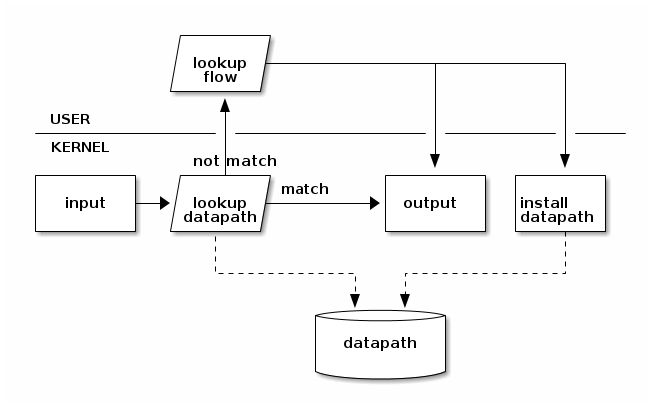
\includegraphics[height=3.5in]{ovs_work_procedure.png}\relax
    \caption{OVS工作流图}
\end{figure}

当Open vSwitch的一个接口收到数据包后,会按照上述流程图处理:收到数据包后,会交给datapath内核模块处理,当匹配到对应的datapath 会直接输出,如果没有匹配到,会交给用户态的ovs-vswitchd查询flow,用户态处理后,会把处理完的数据包输出到正确的端口,并且设置新的datapath规则,后续数据包可以通过新的datapath规则实现快速转发。

\section{基于Coflow的大数据网络优化}
\subsection{coflow相关知识介绍}
另外考虑到当前数据中心用并行计算的框架处理大规模的数据,有人提出了coflow的概念。coflow是一组相关的并行数据流的集合,coflow的完成时间由最后一条数据流的完成时间决定。

\begin{figure}[!htb]
    \centering
    \let\c@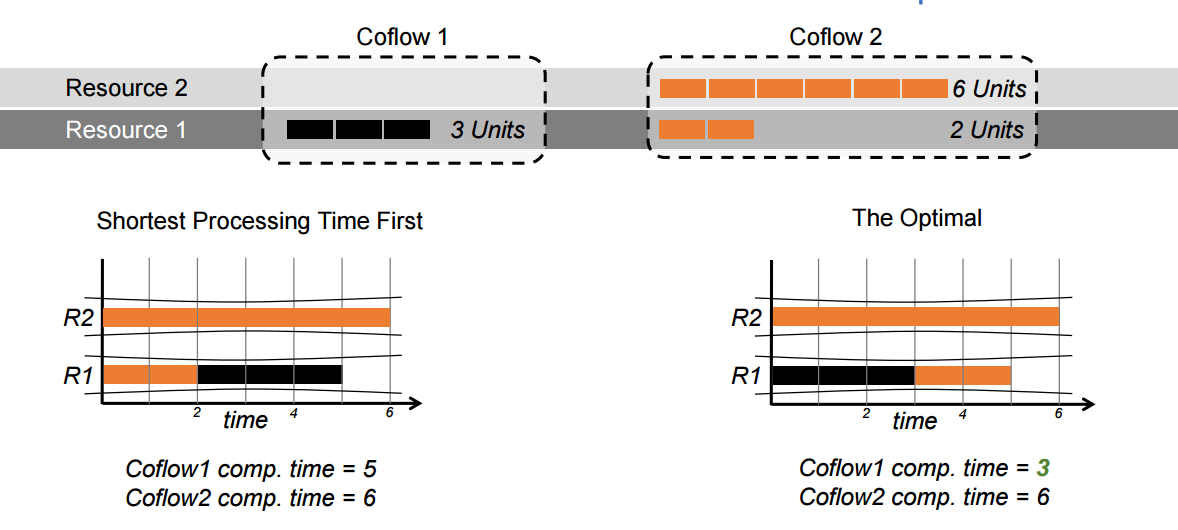
\includegraphics[height=2in]{coflow_cct.png}\relax
    \caption{coflow完成时间的比较}
\end{figure}
此处可详细说明一下这个例子\\
有人设计了varys来提高大数据处理过程中网络通信的性能,他们以最小化完成时间和满足deadline为目标实现了FIFO、SCF和SEBF等启发式算法。采用varys 仿真器coflowsim完成Facebook真实数据的调度测试。\\
coflow研究现状中存在的问题:
\begin{enumerate}
  \item 当前coflowsim中的调度策略都假设所有的flow都是同时出现,不太符合实际情况
  \item 当前的各种启发式算法都是在coflowsim中实现的,还没有用varys调度真实的Facebook数据流,
  \item 当前coflow的两层架构:inter-transfer负责多个transfer间的资源调度,intra-transfer负责一个transfer内的调度。inter-transfer策略主要是加权共享,并没有考虑多个flow间的dependency。
\end{enumerate}
\subsection{coflow调度算法设计}
介绍我们实现的coflow调度算法\\
考虑路由\\
路由算法,最短路径路由,
负载均衡/ECMP/多路径路由\\
varys是交换结构,考虑无阻塞的情况。\\
用matlab仿真,跑一些简单的结果,分析性能

\section{实验平台搭建}
\subsection{实验环境}
\begin{figure}[!htb]
    \centering
    \let\c@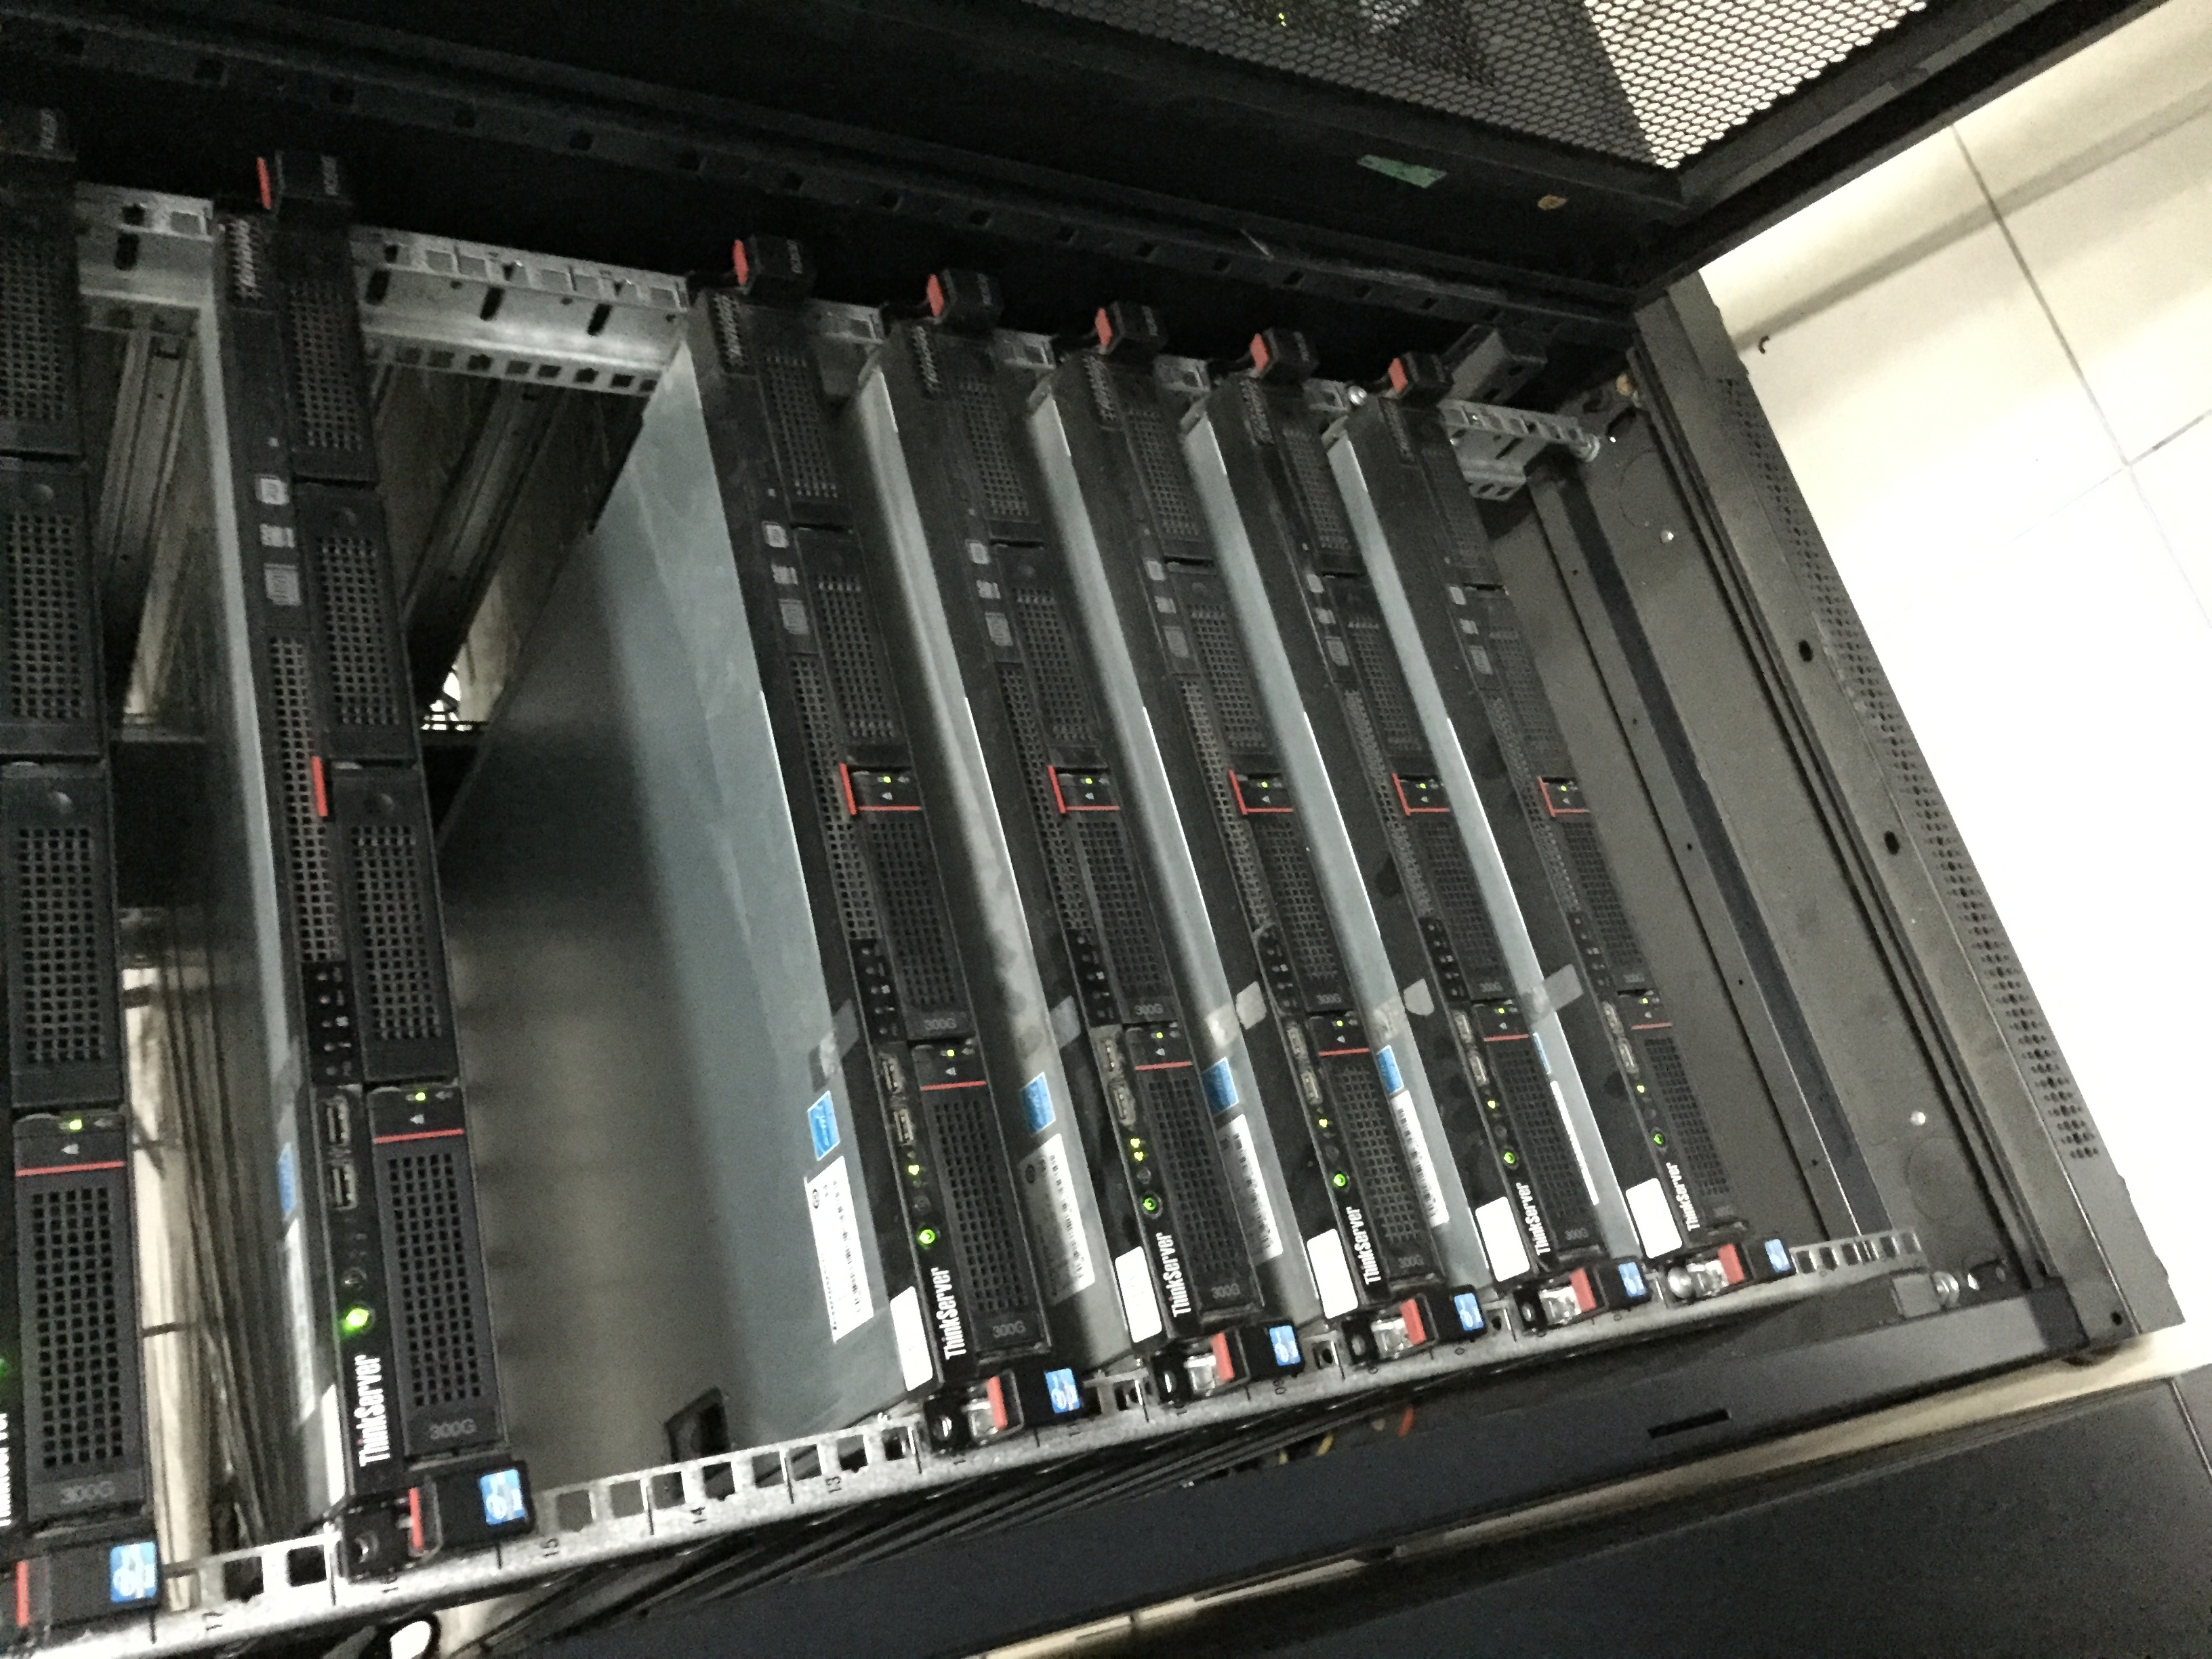
\includegraphics[height=2.5in,angle=-90]{experiment_environment1.JPG}\relax
    \let\c@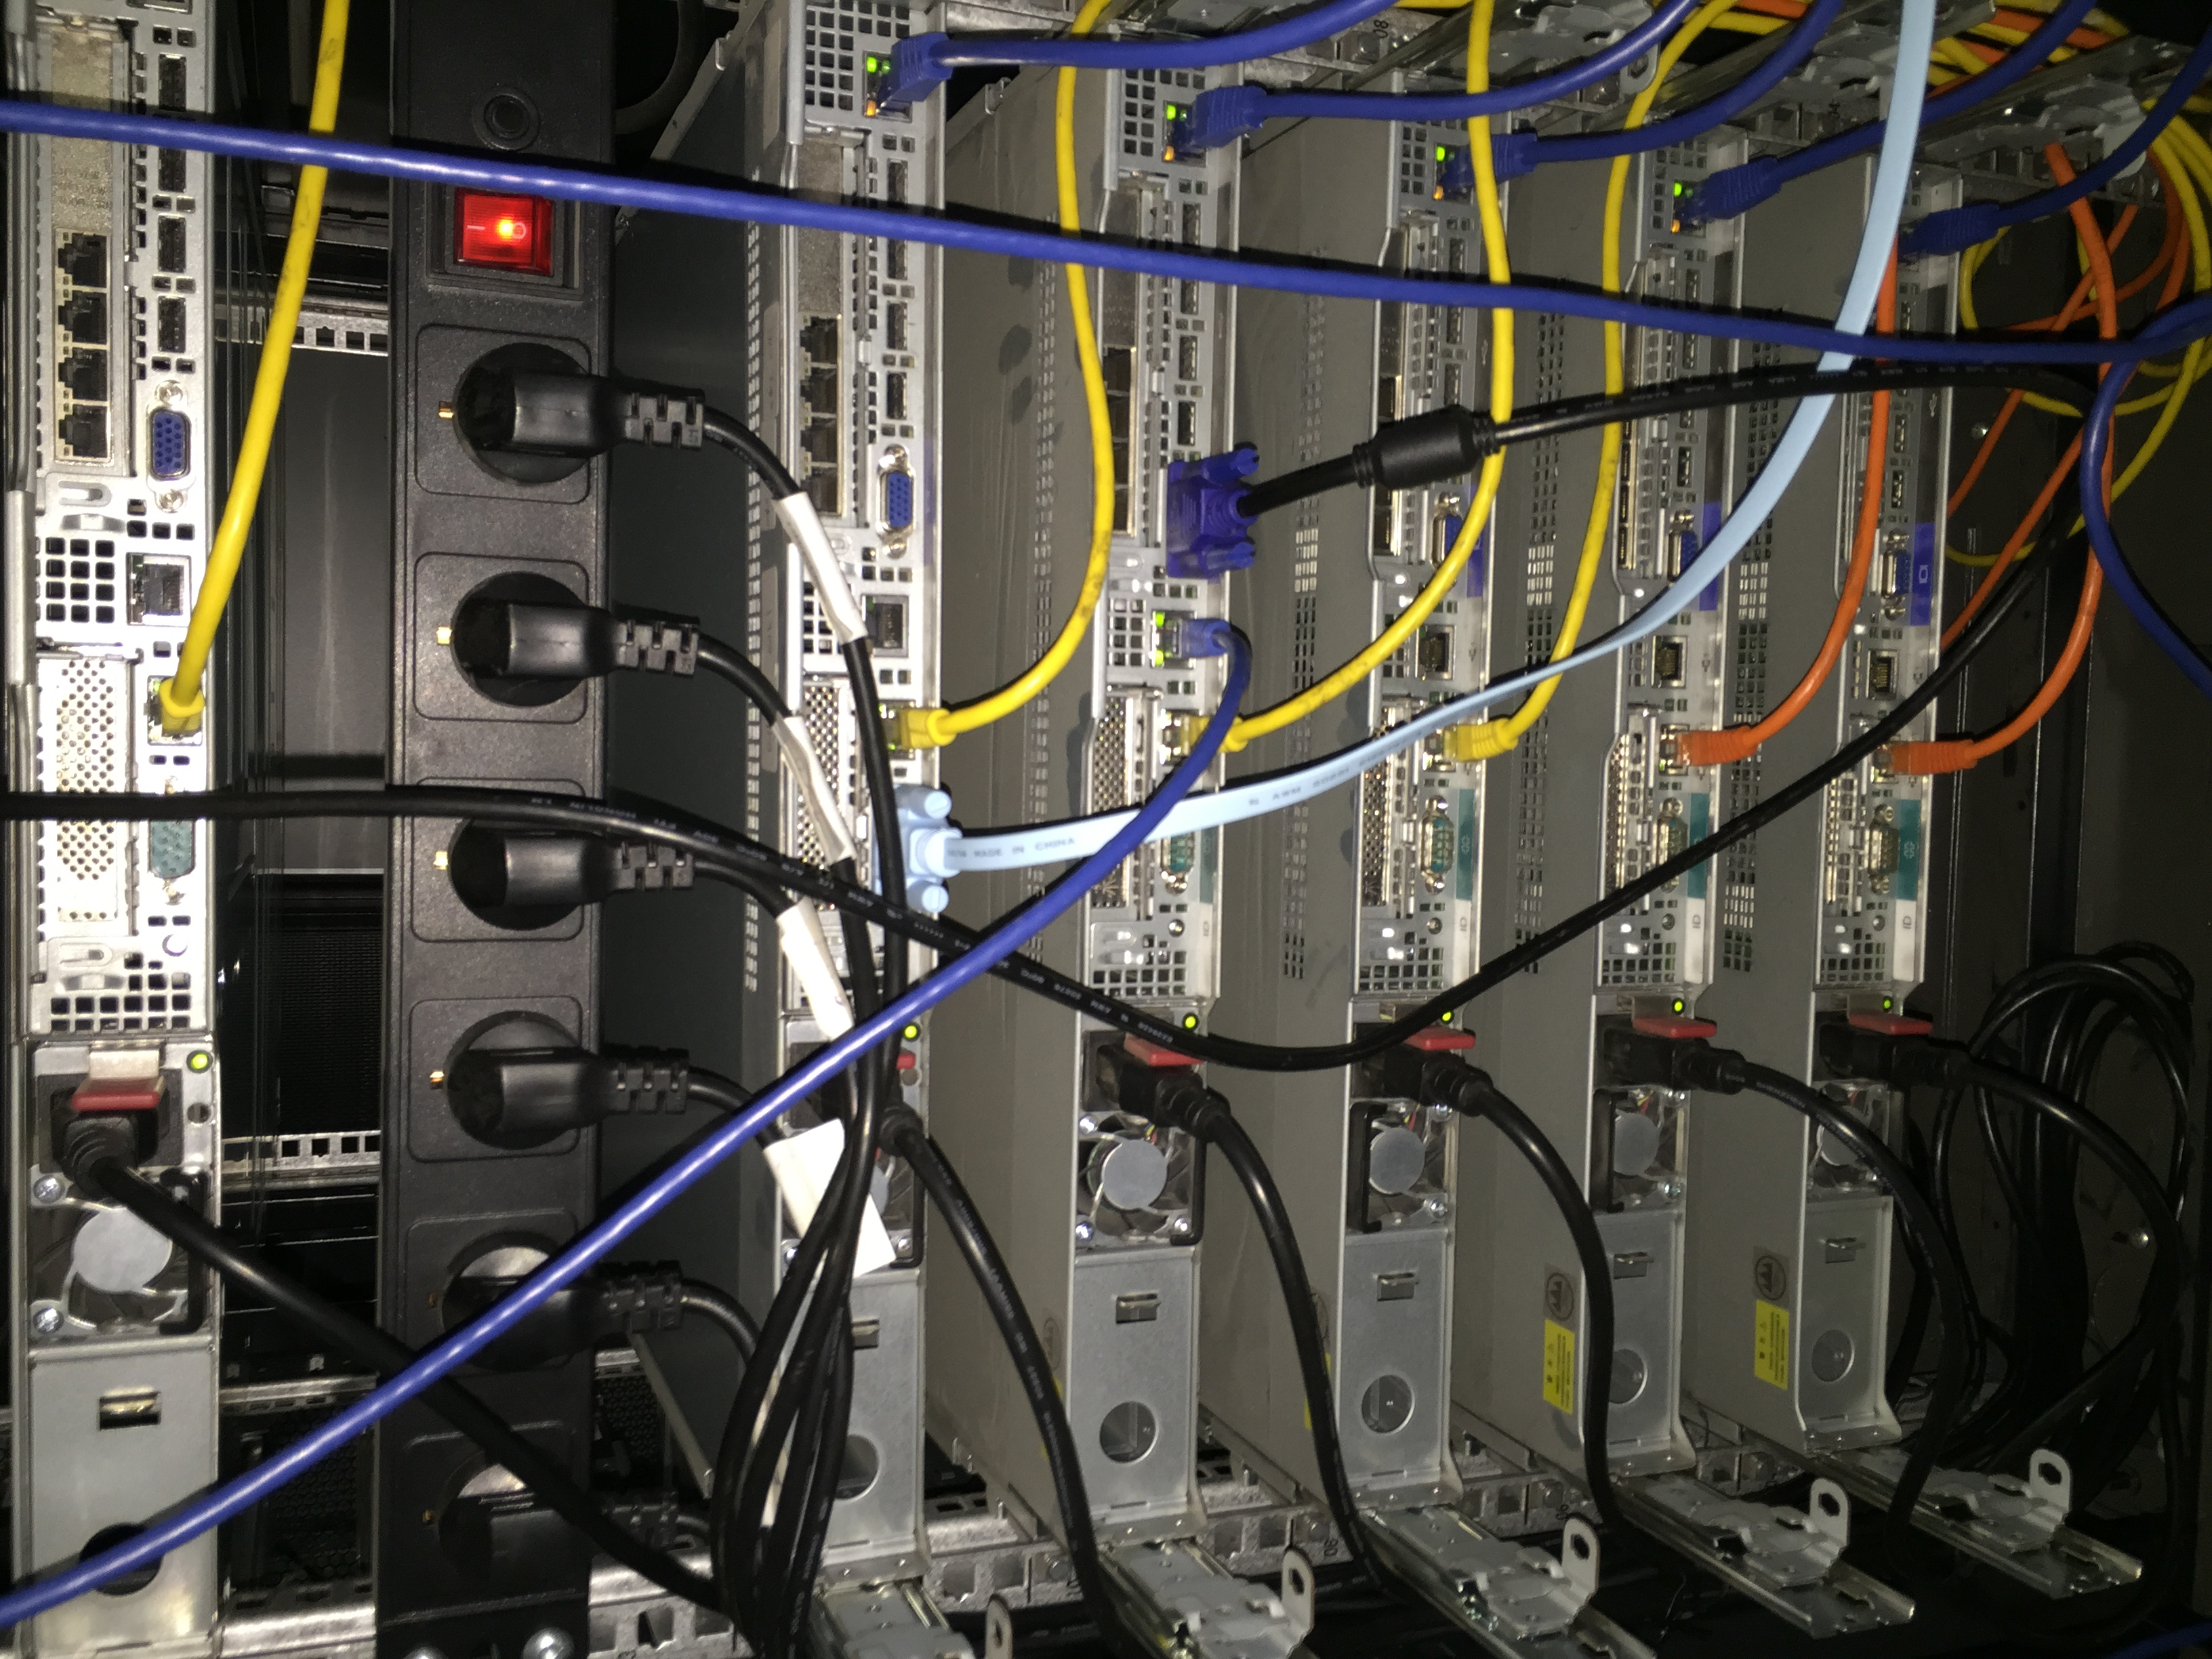
\includegraphics[height=2.5in,angle=-90]{experiment_environment2.JPG}\relax
    \caption{真实的实验环境}
\end{figure}
服务器的性能:机器的型号,内存大小,网卡

\begin{table}[ht]
\caption{系统软硬件及协议配置} \label{table:confg}
\centering
\begin{tabular}{|c|c|c|}
  \hline
  % after \\: \hline or \cline{col1-col2} \cline{col3-col4} ...
  名称 &  配置 \\
  \hline
  服务器配置   &  CPU:16 Intel(R) Xeon(R) CPU\\
             &    E5620 @ 2.40GHz\\
             &    MEM:64G\\
             &    DISK:1000G\\
             &  网卡: 1000 Mbps\\
  \hline
  软件及协议 & Linux ubuntu 14.04 \\
             & Floodlight V1.0\\
             & OVS v2.02 \\
             & OpenFlow1.3 \\
             & Hadoop2.7    \\
             & Python2.7    \\
  \hline
\end{tabular}
\end{table}

\subsection{Hadoop平台搭建}
搭建了hadoop平台,完成多节点的配置,进行大数据的处理
\subsection{SDN开发环境搭建}
搭建基于floodlight的SDN开发环境,进行网络的控制;\\

将多个虚拟交换机ovs挂载到了floodlight控制器上\\
\begin{figure}[!htb]
    \centering
    \let\c@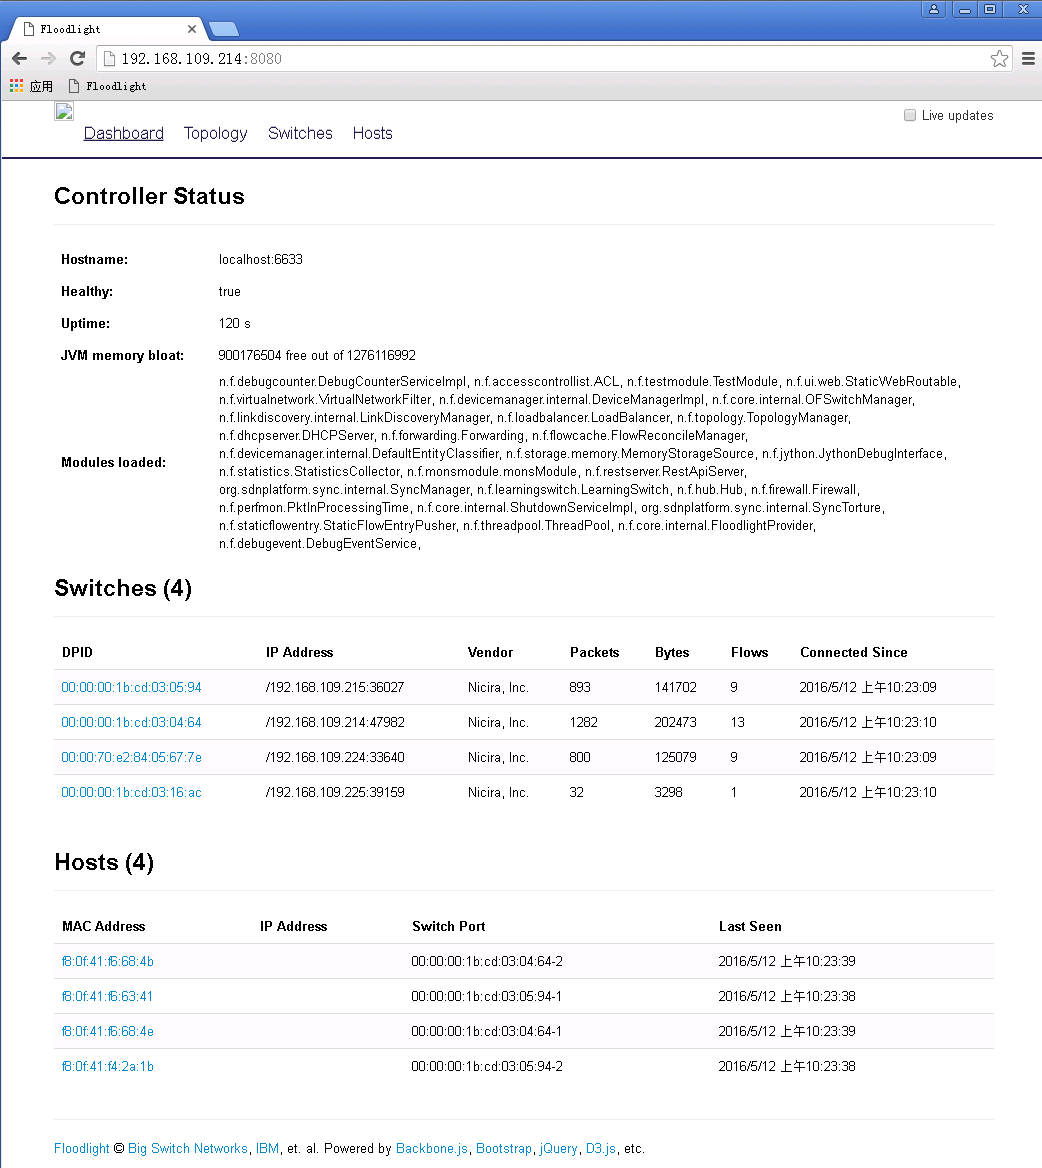
\includegraphics[height=3.5in]{FL_Web_UI.png}\relax
    \caption{Flooglight的Web界面}
\end{figure}

利用ovs完成hadoop平台上的数据导流工作

\subsection{网络拓扑}

\begin{figure}[!htb]
    \centering
    \let\c@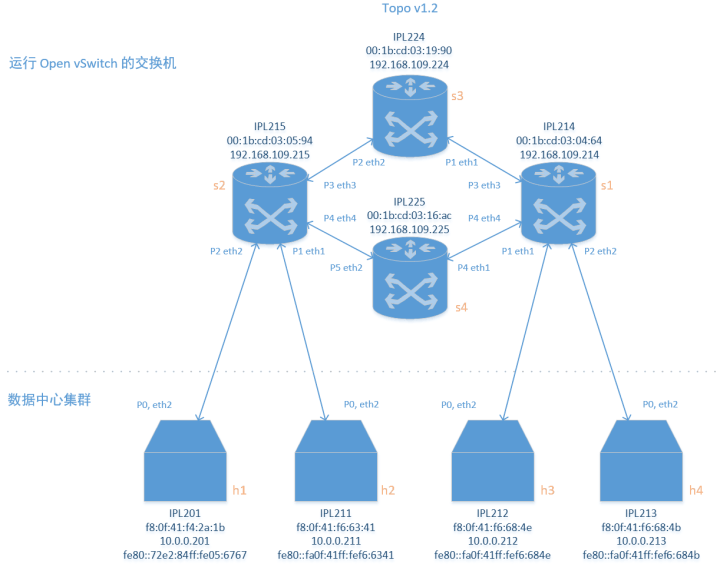
\includegraphics[height=3.5in]{topology.png}\relax
    \caption{网络拓扑结构}
\end{figure}


\section{系统设计与开发}
\subsection{系统整体架构设计}

\begin{figure}[!htb]
    \centering
    \let\c@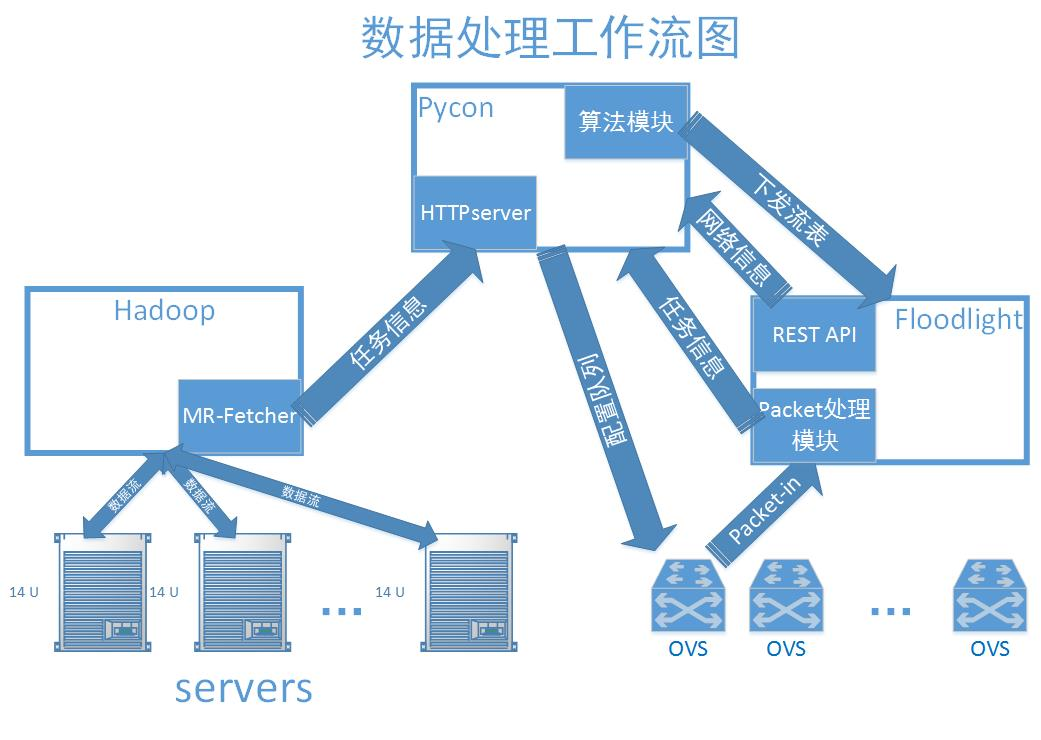
\includegraphics[height=3.5in]{work_arch.jpg}\relax
    \caption{基于SDN+Hadoop的系统架构设计}
\end{figure}

\subsection{Mapreduce Fetcher}

Map任务结束之后,主要进行Copy、Sort、Reduce三个步骤;其中Copy阶段,就是从执行各个Map任务的节点获取map的输出文件。这是由ReduceTask.ReduceCopier 类来负责。ReduceCopier对象负责将Map函数的输出拷贝至Reduce所在机器。在这个过程中,Reduce 进程会启动一些数据复制线程 (Fetcher),通过 HTTP GET 方法请求由 HTTP Server 管理的 Shuffle 数据块,这些数据块是先前成功完成的 Map Task 的输出文件。这些等待 Shuffle 的数据块可能在内存中也有可能在 HDFS 中,取决于服务器当前的内存是否充足以及对 Hadoop 的配置。如果大小超过一定阈值就写到磁盘,否则放入内存。\\
为了利用SDN controller建立全局的调度策略,优化代码插入位置,在NM获得全局调度信息而不用这样一个一个发送,以提高效率。我们做出了一个初步可用的 HTTP Client POST,向PyCon控制器(SDN controller)POST必要的数据,如:源主机、目的主机、数据长度以及MapID等信息。

\subsection{Python Controller(PyCon)}
\subsubsection{HTTPServer 类}

在 Hadoop 中很多地方都用到了 Servlet,并且使用 Jetty 作为 Servlet 的容器来提供HTTP的服务,其主要是通过 org.apache.hadoop.HTTP.HTTPServer 类实现的,HTTPServer 类是对 Jetty 的简单封装,通过调用 HTTPServer 类的 addServlet 方法增加可以实现增加 Servlet 到 Jetty 的功能。\\
 Hadoop 各个组件都会用到 HTTPServer, datanode/namenode, resourcemanager等。\\
Hadoop 内嵌了 HTTP 服务器 Jetty,主要有以下两方面的作用
\begin{enumerate}
  \item 基于 REST API 的 Web 访问接口,用于展示 Hadoop 的内部状态
  \item 参与 Hadoop 集群的运行和管理
\end{enumerate}

\subsubsection{配置队列,进行限速}
为了实现最小瓶颈算法,我们编写了一个 OVS 队列配置模块,可以在 PyCon 启动时自动完成队列的配置操作,以供算法使用。

\subsubsection{获取网络信息}
采用 Floodlight REST API 获取当前受控制的 SDN 网络的带宽使用信息等。不过,直接调用 REST API 获取到的信息不是直接可用的,而是一个 JSON 格式的文本串。我们编写了一段程序将其自动转化为便于处理的矩阵形式。

\subsubsection{流表预配置}
SDN 网络配置流表相比较常规网络较为缓慢,因为当一个数据包没有匹配的流表,交换机会将数据包发送到控制器来请求得到一个回应,得到回应之后才能继续发送数据包,这个过程的延迟较大,大约是 ms 级别的延迟,这对于常规延迟要求较低的 TCP 网络来说是无法容忍的。在我们实际测试的过程中也发现,如果不进行一个流表的预配置,由于延迟较高,TCP 发送端将认为数据包丢失,会进行数据包重传,且较为严重(大约占到 Shuffle 流量的六分之一)。为了缓解这个问题,我们灵活采用 FL API 获得的拓扑信息对网络进行了分析,在交换机上预配置了一系列的流表。大大缓解了实际 SDN 网络中运行传统应用时的数据包重传问题。

\subsubsection{下发流表}
使用 Floodlight 的 StaticFlowPusher REST API 进行流表的下发。默认超时时间是 5 秒,以避免流表过多匹配效率下降的问题。

\subsubsection{路由算法模块}
我们从修改过的 Hadoop Fetcher 模块和 Floodlight 控制器货物获取即将开始传输的 Flow 的信息,然后调用路径计算模块进行路由规划。目前,PyCon 路径计算模块实现了以下两种路由算法:\\

1.加权最短路径算法\\
思路:先使用 Floodlight 的 API 获得当前整体网络带宽使用信息,然后将返回的信息处理成矩阵,以带宽作为权重,调用 Dijkstra 进行计算,得到一条路径。\\
\bigskip

2.最小瓶颈算法\\
思路:要使 Flow 的传输时间最短。计算一条流在网络中所有可行的路径,选择一个带宽最大化,传输时间最短的路径,然后进行流表的下发。\\

细节:
为了实现带宽最大化,我们使用了 OpenFlow 的队列特性。在 Linux 上通过 OVS 调用内核的 QoS Queue 机制实现。队列的配置由 PyCon 完成,不经过 Floodlight。

\subsection{对 Floodlight 的改进}

\subsubsection{Packet-in 数据包处理模块}

Packet-in 数据包是 OpenFlow 协议中当交换机没有对应的匹配流表时,自动向控制器发送的一个数据包,目的是为了获取有效的路由信息,得到控制器的回复之后就可以按照指令传送数据,使数据包可以被顺利发送。

思路:配置流表,让特定数据包以 Packet-in 包的形式传到 Floodlight 控制器。我们编写了一个新模块,使得我们可以顺利提取到 Hadoop Fetcher 无法拿到的端口信息。\\

具体做法:添加了一个 packet-in 数据包处理模块。可以提取 TCP Source Port 和 Payload 内的 Request URI 并且发送给 PyCon,之所以这么做是因为在 Hadoop MR 模块源码内无法通过 HTTPURLConnection 直接拿到 Source Port\\

\subsubsection{REST API}
我们使用了 Floodlight 提供的众多开放的 API,比如拓扑信息,Host 信息,网络速率,流表下发与删除等。\\
但是,由于 Floodlight 目前扔在进一步开发中,功能并不完善。我们额外采用了 OVS 的一些特性进行一些特殊操作,比如直接对 OVS 交换机进行流表操作而不经过 Floodlight,这样我们得以实现一些特殊的功能比如下发 actions=normal(Floodlight 无法直接下发之类特殊操作)。

\section{项目的成果}
\subsection{实验仿真测试}

\begin{figure}[!htb]
    \centering
    \let\c@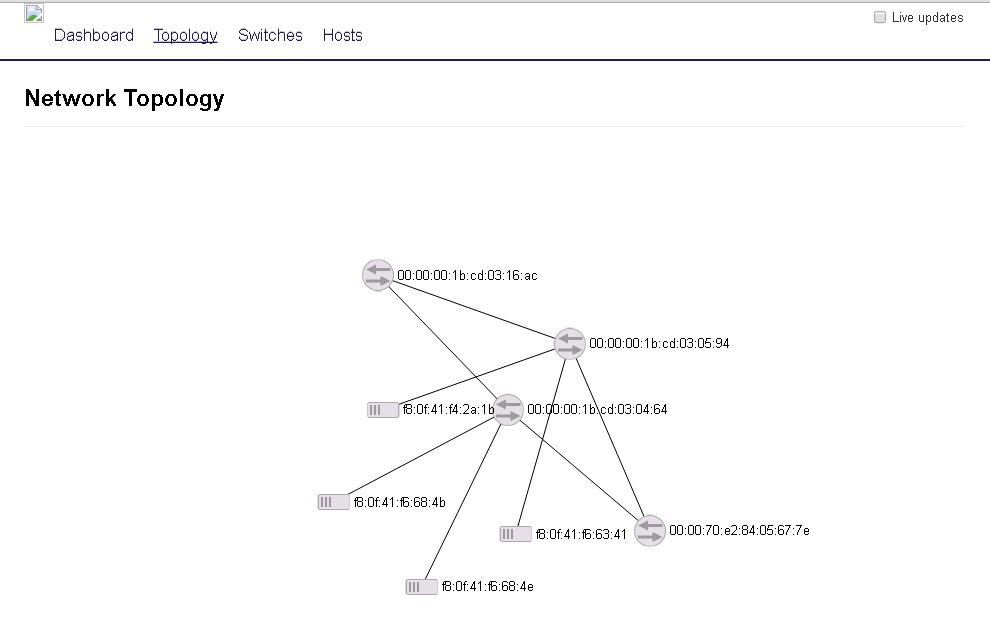
\includegraphics[height=3.5in]{real_topo.png}\relax
    \caption{实验测试网络拓扑结构}
\end{figure}

\begin{figure}[!htb]
    \centering
    \let\c@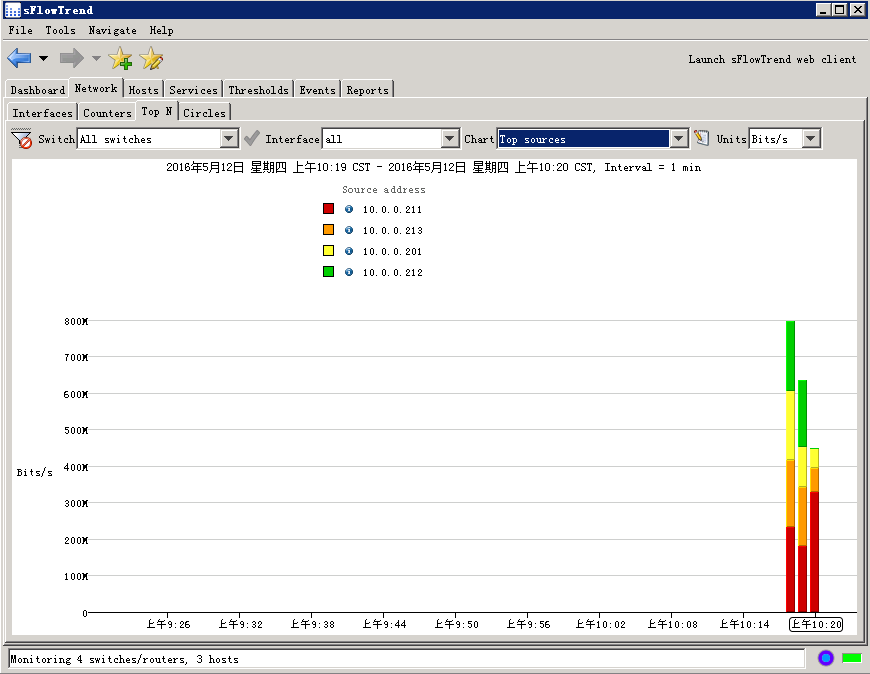
\includegraphics[height=3.5in]{host_real_flow.png}\relax
    \caption{服务器上的实时流量状况}
\end{figure}

\begin{figure}[!htb]
    \centering
    \let\c@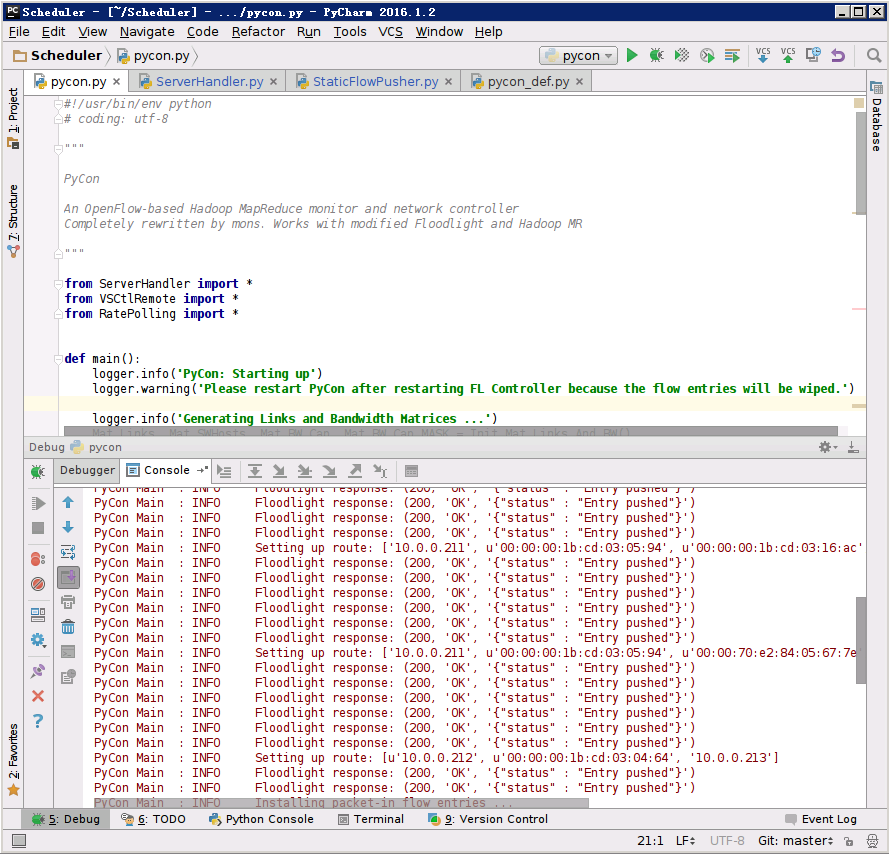
\includegraphics[height=3.5in]{PyCon_running.png}\relax
    \caption{PyCon的运行情况}
\end{figure}

\subsection{实验结果}
由于我们主要进行的是 Hadoop 的 Shuffle 网络优化,我们选择了实际应用和测试中网络传输量最大的 TeraSort 进行测试。\\
TeraSort 是 Hadoop MapReduce 上的一个典型的采用 Map-Reduce 架构的范例程序。通常的大规模数据集群中也会采用 1TB(1024GB) 的数据集大小对数据中心性能进行测试。但由于我们的系统规模不大,仅4 台服务器与4台交换机,并且是在新颖的 SDN 架构上对 Hadoop 大数据应用的研究,我们采用的数据集大小仅为 4GB。

实验参数:数据中心内部所有连接速率均为 1 Gbps,关闭了 MapReduce 的 Map 数据压缩选项,生成排序内容时的数据分块大小为 4(对应 4 台 Host)。实际排序时,所使用的 Map Container 的数量为 32 个(视为 32 个分块)。

由于我们是在测试 SDN 对整体应用性能的优化效果,我们对 TeraSort 排序的总运行时间进行了测定,从提交任务、分配任务到 Reduce 结果返回结果。实验结果表明,未启用 PyCon 时,完成数据排序的时间平均为 203 秒;启用 PyCon 后,数据排序操作时间平均为 193 秒,约有 5\% 的性能提升。

\subsection{结果分析}
提升性能的因素有以下几点:
缓解了直接套用 SDN 网络而不进行有效配置时 TCP 重传导致的网络拥塞;
Floodlight 默认并不会进行负载均衡操作,而 PyCon 采用的算法集成了负载均衡的功能,使得传输效率大大提升。

性能提升并不显著的原因:
% Hadoop 本身对于常规 TCP 网络的优化工作已经较为到位;
由于测试规模受限,数据集较小,无法显著体现优化的性能;\\
实际数据中心内部的带宽普遍较大(1 Gbps),普遍在 100MB 以内数据块的传输只需要 1 秒以内就可以完成,即使只走 1 条路,也只需要多几秒便可以传输完成;\\
在 Reduce 阶段,有且仅有一个容器可以进行工作,进行各个排序子块数据的合并,导致 Reduce 步骤本身在整个任务运行时间中所占的比重较大,而传输时间是一个小量。

\section{项目总结}
(1).当前coflow中所有的flow都是同时出现的。考虑到实际MR中task的启动时间、map完成时间都是不相同不确定的,带来的现实情况是coflow 中的flow 很大可能是不同时出现的。所以我们想采用simulator完成简单的various-start-time-coflow调度工作
(2). 将上述工作用varys实现,并采用ovs完成数据导流工作,实现整个实际平台的运行,并测试结果,对比分析。
(3).考虑更多的研究方向,如:各个coflow/flow的依赖性,除了network 层面的coflow调度,把task执行联合考虑进来,例如把task尽量放到所需data的机器上。\\
SDN性能瓶颈分析
通过分析sdn网络的工作流程,可知控制器通过响应packet-in消息发送packet-out/flow-mod消息的速度是非常重要的,它的快慢直接影响了控制器拓扑发现,流表下发,mac地址学习能力,甚至整个网络的性能。而且SDN网络中通常采用反应式流安装,控制器的响应时间直接影响着流安装的处理速度,本文将重点测试在负载不同的情况下控制器处理packet-in消息的吞吐量和响应时间。同时也关注控制器支持创建openflow连接的能力与拓扑更新的速度。
\section{参考文献}

\bibliographystyle{plain}
\bibliography{references/reference}
%[1] J. Dean et al. MapReduce: Simplified data processing on large clusters. In OSDI, pages 137–150. 2004.\\
%[2] A. D. Ferguson et al. Participatory networking: An API for application control of SDNs. In SIGCOMM. 2013.\\
%[3] Jain S, Kumar A, Mandal S, et al. B4: Experience with a globally-deployed software defined WAN[C] ACM SIGCOMM Computer Communication Review. ACM, 2013, 43(4): 3-14.\\

%\cite{引用文章名称}
%"引用文章名称" 就是前边定义@article后面的名称.

%  \begin{figure}[!htb]
%    \centering
%\subfigure[国外]{\includegraphics[height=3in,width = 2.5in]{clipboard.png}}
%\subfigure[国内]{\includegraphics[height=3in,width = 2.5in]{Wearable.jpg}}
%        \caption{国内外监测身体状况的可穿戴设备及厂商概览}
%\end{figure}
%  \begin{figure}[!htb]
%    \centering
%    \let\c@\includegraphics[height=1.5in]{anyi.jpg}\relax
%    %\let\c@\includegraphics[height=1.2in]{fitbit.png}\relax
%        \caption{needfinding采访}
%\end{figure}
%\section{Brainstorming}
%
%%\begin{figure*}[t!]
%%    \centering
%%    \begin{subfigure}[t]{0.5\textwidth}
%%        \centering
%%        \includegraphics[height=1.2in]{iWatch.png}
%%        \caption{iWatch}
%%    \end{subfigure}%
%%    ~
%%    \begin{subfigure}[t]{0.5\textwidth}
%%        \centering
%%        \includegraphics[height=1.2in]{fitbit.png}
%%        \caption{Fitbit}
%%    \end{subfigure}
%%    \caption{腕带类可穿戴设备}
%%\end{figure*}
%\begin{figure}[!htb]
%    \centering
%    \let\c@\includegraphics[height=1.2in]{iWatch.png}\relax
%    \let\c@\includegraphics[height=1.2in]{fitbit.png}\relax
%        \caption{iWatch and Fitbit}
%\end{figure}


%\begin{figure}[!htb]
%  \centering
%  % Requires \usepackage{graphicx}
%  \includegraphics[width=1.0\textwidth]{objective-function.eps}\\
%  \caption{objective function}\label{eps:o_f}
%\end{figure}
%\begin{figure}[!htb]
%  \centering
%  % Requires \usepackage{graphicx}
%  \includegraphics[width=1.0\textwidth]{classification-Error.eps}\\
%  \caption{classification Error}\label{eps:classification-Error}
%\end{figure}

%%%%%%%%%%  参考文献  %%%%%%%%%%

\clearpage
\end{CJK*}                                     % 结束中文字体使用
\end{document}                                 % 结束全文
